\section{Introduction} \label{sec:intro}
Having  been asked to look at Telescope and Site Software (TSS) after our review in Feb 2018  there are  one or two insights which should be shared.


\section{Code vs  Graphical Interface }

There are basic {\em truths} which we all hold {\em incorrectly} as empirical. I am a programmer I seldom touch a GUI unless I have to. I first saw this explained by Chris Beaumont in Vienna in 2014(\figref{fig:gspec}).
\begin{figure}
\begin{center}
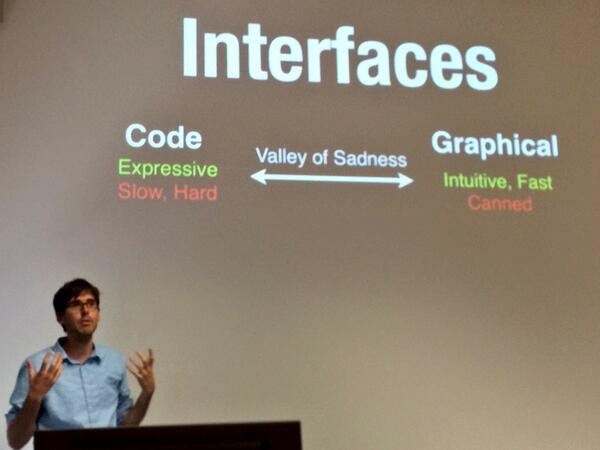
\includegraphics[width=0.6\textwidth]{beaumontCG}
\caption{Code and Graphics - Chris Beaumont Vienna 2014. \label{fig:gspec}}
\end{center}
\end{figure}

I had not thought much about this before but this talk crystallized it for me. I do make occasional plots and diagrams to explain things but it is not the norm. My mistake was to think all programmers are like this. Worse that all smart users were like this.
As with most things there is a spectrum as as in \figref{fig:gspec}, there are a range of approaches and people who use them.

TSS approach seems very graphical with an over  reliance on GUIs.
LabView is inherently graphical, many of us are biased against it\footnote{The license fees do not help}.
However  this goes deeper. Looking at the OCS code this also assumes a GUI, every action like {\em StartNight} is assumed to be an action in a GUI\footnote{Actually it is assumed to be a state which is strictly true but semantically unclear. }.
There seems no way to call this from a script or command line. It seems naive to think we may be able to encapsulate this in a compiled routine\footnote{In Java} anytime before operations.


The LSST users, especially in commissioning, are highly efficient in abstract thinking, scripting and coding of one form or another. There has, perhaps,  been  a major misunderstanding of what users want from the control system. The TSS approach seems to be to provide canned high level procedures (right of \figref{fig:gspec}), the users want and need a much more open and flexible system.
The flexibility is totally necessary in commissioning.
The canned approach is appropriate in later operations, but we have  a lot of AIT and commissioning to go through first.
Right now we do not know the list of procedures, even if we had the list we could not detail how to do them without going through commissioning - the first need is a scriptable system for commanding the observatory (left of \figref{fig:gspec}.


\section{Predicting State}

The second philosophical approach is toward state or the ability to know state. There is a basic principle in the TSS architecture that everything is  Finite State Machine (FSM).
Since the observatory is a series of machines this is strictly true, however we do not know all the possible states or modes of the machine(s) and we probably will not know them until well into operations.
We will begin to learn this in commissioning. There has been a major conflict with  TSS team seeking the {\em requirements} from the T\&S team for several years.  LSST is complex and has some novel aspects, I believe TSS are looking for the full set of modes and states for LSST - I also believe it is impossible to know that for an as yet built system like LSST. Hence can one ever build an FSM for operations it before it is complete ?

The FSM is the {\em correct} approach  but it can not be applied system wide. We all fall in the trap of generalization.
In this case trying to apply the FSM approach to the entire system will never work and has locked the TSS team up in an impossible task -
the team has been waiting for the requirements (which define states) ) while many of us understand we will not know those states until we are on the mountain with the actual hardware.

The FSM approach is inherently restrictive  it allows one to do exactly what is prescribed. A new observatory like LSST, especially in commissioning, needs a much more flexible and open approach. A very restrictive system with only {\em allowed} transitions often leads to ta situation where {\em the system} will not allow an activity even if the users/engineers/observatory scientist agree it is the correct action. Again this is probably ok in operations but not in commissioning.

For Example, at some point we will need to manipulate the louvers to control air flow.
 How we do that will depend on wind and temperatures - we do not know today how that will be done.
There will probably be some formula taking account of temperature inside the dome and airflow outside the dome.
Initially  we \footnote{The royal we here is really the commissioning team and operators.} will possibly adjust the louvers until we understand how they work over many nights, we may experiment with a number of formula looking at EFD and sending SAL commands.
 This requires a very flexible system,  not an FSM though of course once could make a more flexible FSM.

\section{Conclusion}
In TSS we need to focus on a flexible programmable interface to meet the  primary needs of AIT and Commissioning.
Meanwhile we have an INRIA contract to build a graphical interface for Operations (and possibly some of commissioning).
This of this very much in the terms of hackable user interface \citep{2015ASPC..495..101B}.
We also do need to be aware of the safety of operating the system - as we build up scripts for testing, AIT and Commissioning we will start to build more constraints into the system - we should not try to build all constraints in from the start.


